\section{agenda}

%%%%%%%
%\captionsetup{labelformat=empty} % 
\begin{center} % to remove Fig.
    
\begin{tikzfigure}[]
%\begin{minipage}[b]{1\linewidth}

%Taiwan\\
%\vspace{5cm}
\includesvg[height=2.0cm, distort=false]{Flag_of_Somaliland.svg}
\hspace{2cm}
%\includesvg[width=0.17\linewidth]{TMM_logo.svg}
%\hspace{3cm}
\includesvg[height=2.0cm, distort=false]{Flag_of_the_Republic_of_China.svg}
%\captionof{Figure}{xx}
%\end{minipage}
\end{tikzfigure}

\end{center}


%%% title; font size and baseline offset (line space)
\fontsize{20}{24} \sc
2024 Collaborating for Public Health: \\
A Multi-Specialty Conference \\
%on Taiwan and Somaliland
 \par
\vspace{0.3cm}
% FOR MINISTRY OF HEALTH DEVELOPMENT

\fontsize{12}{13} \sc
Taipei Municipal Wanfang Hospital versus Hargeisa Group Hospital\\
On 11 May, 2024, at 09:00 am, Saturday \\
Venue: Conference Hall of Carro Edeg Hotel, Hargeisa
%Exhibition Hall of the Hargeisa Group Hospital
% no more Jees Hotel
\par
%\vspace{0.2cm}
%%%%%%%%%%%%




% agenda
%\begin{columns}

%\column{0.7}
%\block{Agenda}{

\begin{center}
    
%\begin{minipage}{0.9\linewidth}

% Please add the following required packages to your document preamble:
% \usepackage{graphicx}
\begin{table}[h]
\centering
\resizebox{1.00\textwidth}{!}{%
\begin{tabular}{llll}
%%%% day 1 Dr. Tsan-Hon Liou; Dr. Chen-Yuan Chiang
\textbf{11 May} & \textbf{Topic} & \textbf{Speaker} & \textbf{} \\ \hline \hline
09:00 & Opening & \begin{tabular}[c]{@{}l@{}} \textbf{Dr. Tsan-Hon Liou, M.D., Ph.D.}\\(Superintendent, TMWH)\end{tabular}
& \\

%%%%%%
\hline
& \textbf{Session 1: Somaliland Dengue Fever Prevention and Control} & & \\
%09:05 & Somaliland EPHS 2019 Overview & \begin{tabular}[c]{@{}l@{}} \textbf{Dr. Lula Hassan, M.D.}\\(Director General, Ministry of Health Development)\end{tabular} & \\
09:05 & Somaliland EPHS 2020---WHO IEC Materials for Dengue Fever & \begin{tabular}[c]{@{}l@{}} \textbf{Dr. Deq Said Jama, M.D.}\\(Director, WHO Office in Hargeisa)\end{tabular} & \\

09:35 & Clinical Guideline for Dengue Fever Management & \begin{tabular}[c]{@{}l@{}} \textbf{Dr. Adnan Sayid Abdo, M.D.} \\(Deputy Director, Hargeisa Group Hospital, HGH)\end{tabular} & \\

10:05 & Taiwan Cares: Taiwan’s experience in Dengue Fever Prevention and Control & \begin{tabular}[c]{@{}l@{}} \textbf{Dr. Chin-I Chen, M.D., Ph.D.}\\(Director, Department of Preventive \& Social Medicine, TMWH)\end{tabular} & \\

10:35 & Panel Discussion/Eye Relaxation Break & \begin{tabular}[c]{@{}l@{}} \textbf{Dr. Deq, Dr. Adnan, Dr. Chen, and Dr. Chen-Yuan Chiang}\\\end{tabular} & \\
\hline

% 江振源Chen-Yuan Chiang

%%%%%%%%%%%% or breast cancer by Dr. Afnan
%& \textbf{Session 2: Esophageal Cancer and Hepatoma in Somaliland} & & \\

%10:45 & Epidemiology of Esophageal and Liver Cancer in Somaliland & \begin{tabular}[c]{@{}l@{}} \textbf{Dr. Omar Marshal, M.D.}\\(Director of Pathology Department, HGH)\end{tabular} & \\

%11:05 & Esophageal and Liver Cancer Therapy in Taiwan:  & \begin{tabular}[c]{@{}l@{}} \textbf{Dr. Tzeon-Jye Chiou, M.D.}\\(Director of Cancer Center, TMWH)\end{tabular} & \\
% 邱宗傑 Tzeon-Jye Chiou(108178) A Rising Threat in Somaliland
% 血液病及各類淋巴瘤、多發性骨隨瘤、白血病、呼吸道癌、消化系統上、下胃腸道癌及肝、膽道系統腫瘤、泌尿系統癌

%11:05 & Panel Discussion/Eye Relaxation Break & \begin{tabular}[c]{@{}l@{}} \textbf{Dr. Omar and Dr. Tzeon-Jye Chiou}\\ \end{tabular} & \\

%%%%%%%%%%%%%%
\hline
& \textbf{Session 2: Orthopedic Training in HGH and TMWH} & & \\

10:45 & Orthopedic Training Program at HGH & \begin{tabular}[c]{@{}l@{}} \textbf{Dr. Ahmed Saed Ali, M.D.} \\ (Director, Orthopedic Department, HGH)\end{tabular} & \\

11:15 & Orthopedic Training Collaboration between HGH and TMWH & \begin{tabular}[c]{@{}l@{}} \textbf{Dr. Yu-Pin Chen, M.D., Ph.D.}\\(Attending Surgeon, Orthopedic Department, TMWH)\end{tabular} & \\
% Dr. I-Chien Kuo

11:45 & Panel Discussion & \begin{tabular}[c]{@{}l@{}} \textbf{Dr. Ahmed and Dr. Chen}\\ \end{tabular} & \\

\hline
12:00 & Closure/Group Photos/Lunch Break & & \\
\hline
\end{tabular}%
} % end of resizebox


\end{table}


%\end{minipage}

\end{center}



%%%%%%%%%%%

%%% footer
%\block{}{
%\node [above right,
%       outer sep=0pt,
%       minimum width=\paperwidth-2*\pgflinewidth,
%       minimum height=7cm,
%       align=center,font=\Huge,
%       draw,fill=green!30,
%       ultra thick] at ([shift={(0.5*\pgflinewidth,0.5*\pgflinewidth)}]bottomleft) 
%       {

\begin{tikzfigure}[]
%\includesvg[height=40.0cm, distort=false]{ortho_ward_Tex_Josh.svg}

%\includesvg[height=2.5cm, distort=false]{TRO_Somaliland.svg} \hspace{2cm}
%\includesvg[height=2.5cm, distort=false]{MoHD_Somaliland.svg}

%\hspace{1cm} % https://mohd.govsomaliland.org/
%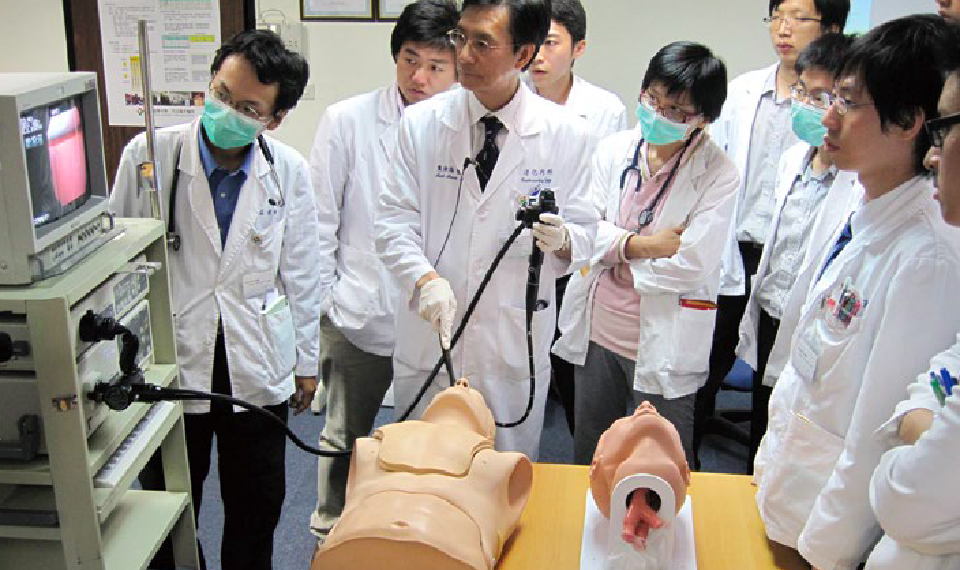
\includegraphics{TMWH_scope.pdf}


%*** using zong Kai Chinese font by \ZongKai{}, and adjust image size \scalebox{h}[v]{}
% image and character: \resizebox{2.7cm}{1.5cm}{}
\ZongKai{\fontsize{3.3}{6}\selectfont \scalebox{1.3}[1.0]{\includesvg[height=1.5cm, distort=false]{TRO_Somaliland.svg}}}
\includesvg[height=1.5cm]{TMWH_logo_TAIPEI_vector.svg}
%\includesvg[height=25.0cm, distort=false]{TRO_Somaliland_font_ZongKai.svg.svg}\hspace{1cm} % TRO logo with ZongKai font in path
\includesvg[height=1.5cm, distort=false]{TMM_logo.svg}
%{2023TMM_officePlate_pink.svg}
\includesvg[height=1.5cm, distort=false]{Hargeisa_Group_Hospital_logo.svg}
%\includesvg[height=1.5cm, distort=false]{MoHD_Somaliland.svg} % 2020
\includesvg[height=1.5cm, distort=false]{logo_MoHD_HGH.svg} 
%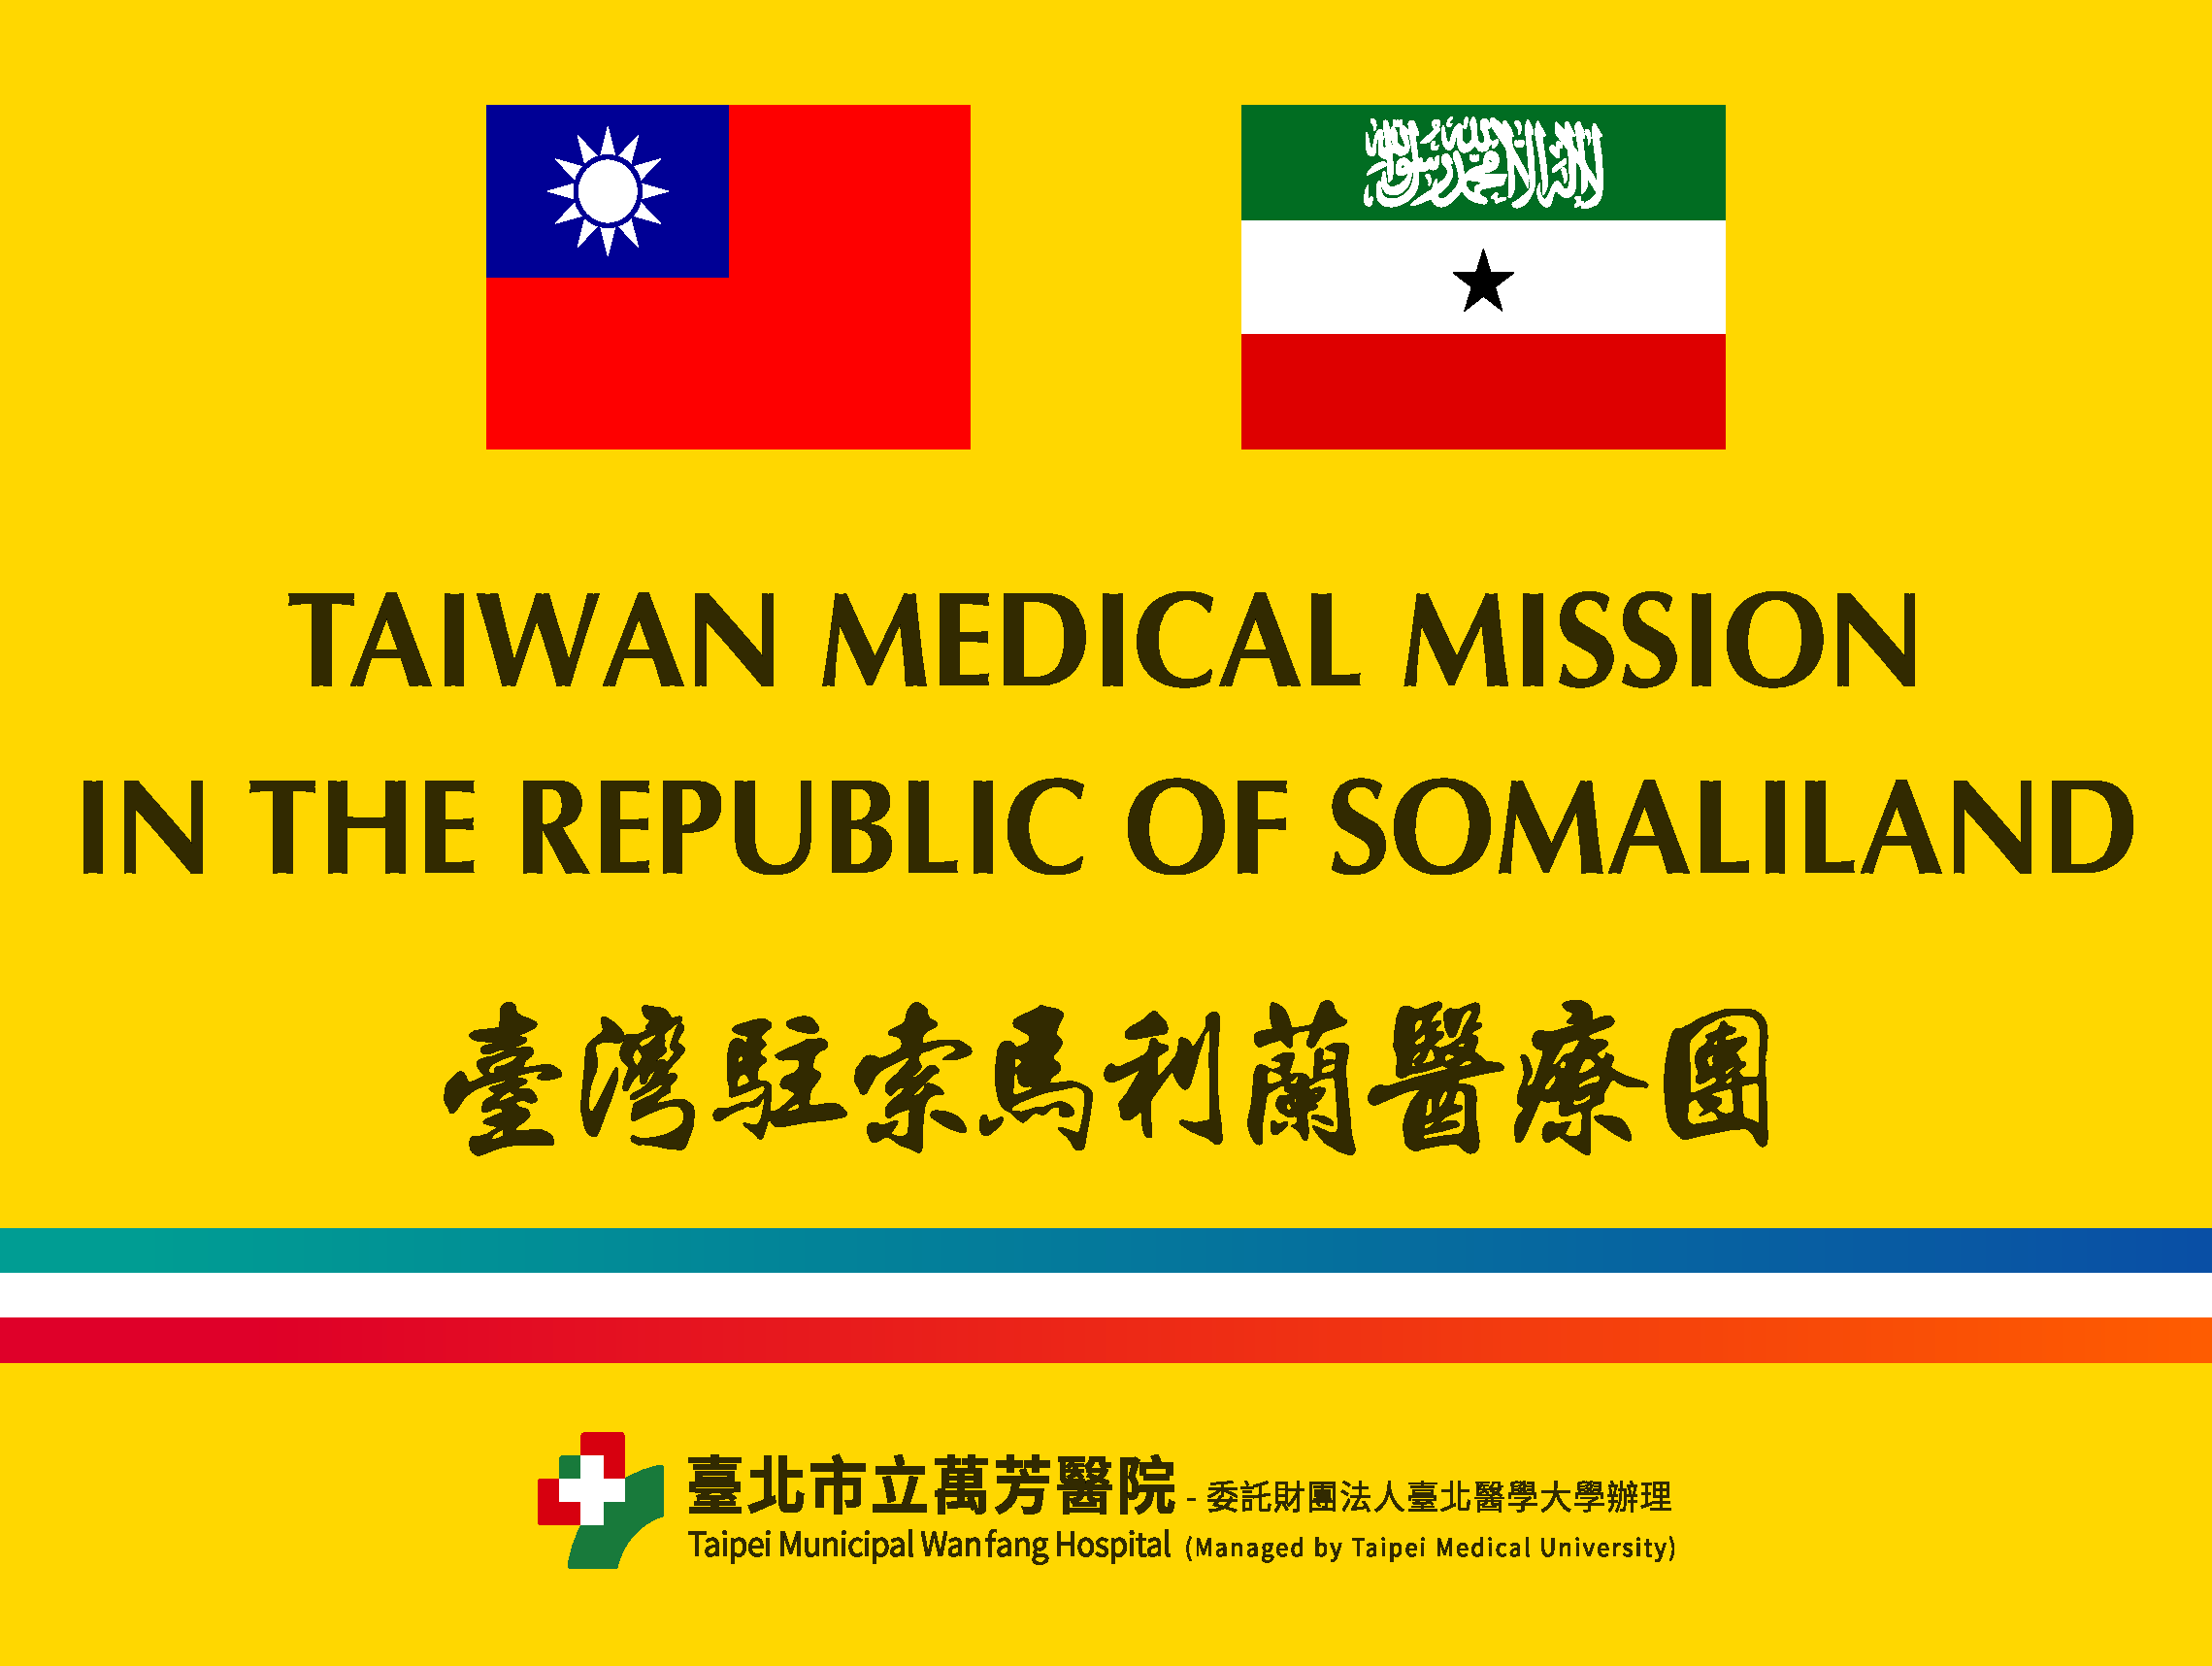
\includegraphics[height=12.0cm, distort=false]{2023TMM_officePlate_ai.pdf}

%%% *********
% ?? add logo of military and social welfare ??

\end{tikzfigure}



%}; % end of node

%} % end of block
